\chapter{Git and github}



\section{Algunas extensiones de VSCode para Git}


\subsection{Git History}

Es una extensión que sirve para visualizar los cambios históricos que se han hecho a los diferentes archivos.

Mediante el comando \texttt{Ctrl+Shift+P} y la opción \texttt{View file History} se abre una ventana que indica las versiones del proyecto (commits) y cómo han sido los archivos al momento de hacer la confirmación de esa versión.

\begin{figure}[H]
    \centering
    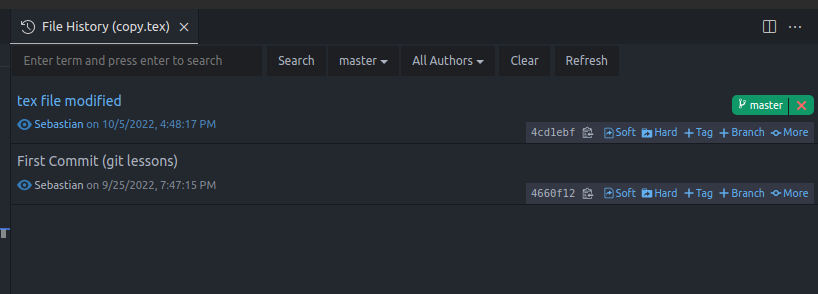
\includegraphics[width=0.6\columnwidth]{Github/Git_f1.png}
\end{figure}


Para cada versión se mostrará el archivo modificado y cómo es su contenido al realizar la confirmación. \\

La siguiente opción es para realizar comparación de ese archivo en esa versión con la actual que está en el espacio de trabajo.

\begin{figure}[H]
    \centering
    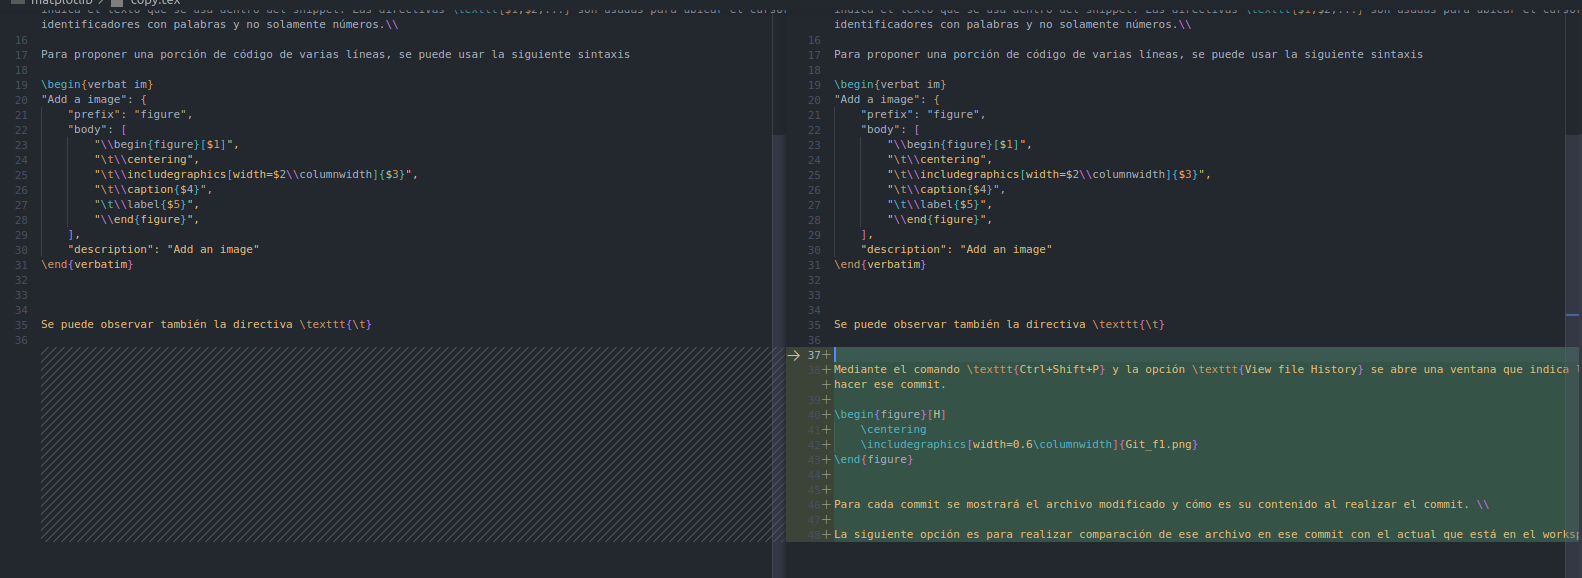
\includegraphics[width=0.6\columnwidth]{Github/Git_f2.png}
\end{figure}

Las siguientes opciones permiten ver la comparación del archivo su versión anterior. Y la última opción permite ver la historia completa del archivo

\subsection{Git Blame}

Esta extensión sirve para realizar revisión línea por línea de por quién, hace cuánto y en qué versión se realizó esa línea de código


\begin{figure}[H]
    \centering
    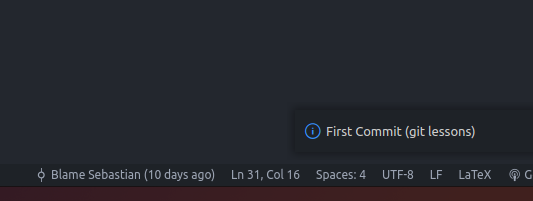
\includegraphics[width=0.6\columnwidth]{Github/Git_f3.png}
\end{figure}


\subsection{Git Lens}

Esta extensión es similar a las anteriores, en que ayuda a verificar las identidades de las personas que están modificando archivos, muestra línea por línea información del autor, y versión de la línea en cuestión.  

\section{Fundamentos de Git: cómo funciona por dentro}

\subsection{Crear un nuevo repositorio}

La sentencia primaria y básica para inicializar un nuevo repositorio es \\

\texttt{git init} \\

Este comando se realiza dentro de la carpeta en la que se desea realizar el repositorio. Una vez creado el repositorio, se pueden añadir las carpetas correspondientes dentro. Al crearse el repositorio, se crea una carpeta oculta llamada \texttt{.git} de manera automática.

dentro de esta carpeta tenemos diferentes carpetas y archivos. Uno de ellos es el archivo \texttt{config}, en este archivo tenemos una serie de cadenas que nos indica las configuraciones que tiene el repositorio. El siguiente es un ejemplo de un archivo de configuración:
\begin{verbatim}
[core]
        repositoryformatversion = 0
        filemode = false
        bare = false
        logallrefupdates = true
        ignorecase = true
[remote "origin"]
        url = https://github.com/JhoAraSan/Process.git
        fetch = +refs/heads/*:refs/remotes/origin/*
[branch "master"]
        remote = origin
        merge = refs/heads/master
\end{verbatim}

Otro archivo es el de descripción \texttt{description}, el cual se puede editar para añadir una descripción al repositorio. Finalmente el archivo \texttt{HEAD}, el cual puede arrojar la siguiente cadena:
\begin{verbatim}
ref: refs/heads/master
\end{verbatim}
Más adelante se dará la explicación correspondiente a este archivo. \\
 Git tiene su propio sistema de archivos; en este sistema de archivos git guarda o almacena objetos, y estos objetos son guardados dentro de la carpeta correspondiente \texttt{objects}.

 \subsection{Objetos en Git}

 En git existen cuatro tipos de objetos:
 \begin{verbatim}
Blob
Tree
Commit
Annotated Tag

 \end{verbatim}
Estos cuatro objetos son los suficientes para poder realizar todo el seguimiento de los archivos del repositorio.
\subsubsection{Blob}
Este es el tipo de objeto en el que git guarda \textbf{archivos}. Todo tipo de archivos con la extensión que sea. Cualquier tipo de archivo serpa guardado como un blob. 
\subsubsection{Tree}
Este es el tipo de objeto en el que git almacena la información sobre los directorios. Dicho de otra fforma, un objeto Tree es una representación de una carpeta o un directorio.
\subsubsection{Commit}
A través de este tipo de objeto, Git es capaz de almacenar diferentes versiones de uno o varios archivos a través del tiempo.
\subsubsection{Annotated Tag}
Este objeto es esencialmente un texto que está apuntando a un commit versión específica. \\

Para poder gestionar o administrar objetos en git se usan los comandos de git de bajo nivel:

\texttt{git hash-object} Con esre comando podemos crear nuevos objetos con la estructura de git.
\texttt{git cat-file} Con este comando se pueden leer los objetos git.
\texttt{git mktree} con este comando se puede crear un nuevo objeto de tipo Tree 

A manera de ejemplo, si colocamos un texto string cualquiera mediante el siguiente comando:

\begin{verbatim}
echo "Hello, Git" | git hash-object --stdin -w
\end{verbatim}

Vamos a obtener como salida un hash, además de que se creará el objeto correspondiente en la carpeta objects; la carpeta será los dos primeros caracteres del hash, y dentro habrá un archivo con el resto de caracteres del hash. Solamente se crea el objeto, el repositorio seguirá estando vacío. Importante remarcar que el hash retornado es el hash del string que le metimos de entrada.

\subsection{JSON}

Las siglas significan "JavaScript Object Notation". Es un formato que permite el intercambio de datos entre diferentes servidores. Como ejemplo, podemos extraer datos mediante una API desde un servidor a una página web. La siguiente es un ejemplo de una estructura JSON:

\begin{verbatim}
{
    "id": "12345667",
    "name": "Mike",
    "age": 25,
    "city": "New York",
    "hobbies": ["Skate", "Running"]
}
\end{verbatim}

Siempre será recomendado que las llaves en un archivo Json sean únicas. La estructura de datos que hay en git es muy similar a JSON; Git tambien almacena nombres "llave" y valores. Las "llaves" en git son los hashes de cada objeto. En git, el hash generado (el cual es equivalente a la key) es función o depende del valor.

\subsection{Hash}

 Al realizar el comando de la seccion anterior, vimos que ek string \texttt{"Hello, Git"} generó un hash \texttt{b7aec520dec0a7516c18eb4c68b64ae1eb9b5a5e}. Esto significa que se aplicó una funcion hash al string o al dato ingresado. \\

 Una función hash es una función que toma una entrada de cualquier tamaño (longitud) y tiene una salida de un tamaño fijo. Es importante también notar que el hash es una funccióon unidireccional, es decir, que si tenemos un hash generado no vamos a poder saber cuál fue la entrada que la generó. Para la misma función hash, la misma entrada siempre va a generar la misma salida. \\

 Las fuciones o algoritmos para generar hashes más importantes son las siguientes:

 \begin{itemize}
     \item MD5 (128 bit)
     \item SHA1 (160 bit)
     \item SHA256 (256 bit)
     \item SHA384 (384 bit)
     \item SHA512 (512 bit)
 \end{itemize}

 El algoritmo usado por git para generar sus hashes es \texttt{SHA1}.

 Cada caracter de 4 bits de longitud está está en formato hexadecimal. Por tanto, un hash de git tiene una longitud de 40 caracteres hexadecimales. \\

 Dado lo anterior, surge la pregunta de cuantos archivos diferentes podemos guardar en el mismo repositorio.

 La cantidad total de hashes diferentes es $16^{40} \approx 1.46 \ 10^{48}$. Por otro lado podemos havernos la pregunta de cual es la posibilidad de que dos archivos diferentes produzcan el mismo hash? \\

 La probabilidad de encontrar un hash específico es $\frac{1}{16^{40}} \approx 6.84 \ 10^{-49}$. Por tanto para saber la probabilidad de que dos archivos produzcan el mismo hash, tenemos \\

 \begin{equation*}
 P = \frac{1}{16^{40}}  \frac{1}{16^{40}} = \frac{1}{16^{80}} \approx 4.68 \ 10^{-97}
 \end{equation*}

Como elemento adicional, tenemos que la probabilidad de que teniendo $n$ archivos diferentes, dos de ellos generen el mismo hash, es el siguiente:

\begin{equation*}
P = \frac{(2^{160}-n)!(2^{160})^{n-1} - (2^{160} - 1)! }{ (2^{160}- n)! \ 2^{160(n-1)} }
\end{equation*}

Para que haya una probabilidad de 1 de que haya una colision de hash es necesario que en un repositorio hayan más archivos que número diferente de hashes. 

\subsection{Exploración de objetos de git mediante \texttt{cat}}

Recordemos que todo objeto de git tiene su correspondiente hash. Podemos usar el comando \texttt{git cat} para obtener información de cualquier objeto. Las opciones del comando son: 

\texttt{git cat-file -p <hash>} Retorna el contenido del objeto. \\
\texttt{git cat-file -t <hash>} Retorna el tamaño del objeto. \\
\texttt{git cat-file -s <hash>} Retorna el tipo del objeto. El tamaño lo retorna en bytes. \\

\subsection{Creación de objetos mediante comandos de git}

el comando \texttt{git hash-object} se usa para crear nuevos objetos, luego tenemos varias opciones adicionales:
\begin{verbatim}
echo "Hello, Git! | git hash-object --stdin -w
\end{verbatim}

La promera opvion es para romar la intrada como entrada estandar, la segunda es importante porque es la que hace se cree el objeto. También podemos crear objetos en git basados en archivos locales:

\begin{verbatim}
git hash-object <filename> -w
\end{verbatim}

Una cosa importante de notar es que en git cuando almacenamos archibos del tipo blob, estos objetos no tienen un nombre de archivo. Como se podrá ver en los anteriores comandos, ninguno de ellos retorna el nombre del archivo puesto que este no se almacena. Otra cosa importante de notar es que tanto el tamaño como el tipo de objeto se almacenan dentro del mismo hash. La estructura con la que lo hace es la siguiente:

contenido + tipo de objeto + tamaño del objeto = hash.  Entre el tipo de objeto más tamaño, y el contenido del objeto hay un delimitador. En esencia, el hash se genera a partir de lo siguiente:

\begin{verbatim}
blob 11\0Hello
\end{verbatim}

El delimitador es \texttt{$\backslash$0}, antes del delimitador tenemos el tamaño que para el ejemplo es 11 bytes, y antes el tipo de objeto seguido de un espacio. Luefo del delimitador está el contenido del archivo. 

\subsection{Tree}

Este tipo de objeto es el que representa las direcciones y los directorios.  Un objeto Tree puede tener tanto blobs como otros trees. La estructura es la misma de los demás objetos (tipo, tamaño, delimitador y contenido). En este caso el contenido será diferencial al de un blob: 

\begin{verbatim}
100644 blob 57537e1d8fba7d80c5bcca8b04e49666b1c1790f .babelrc
100644 blob 602c57ffb51af99d6f3b54c0ee9587bb110fb990 .flow config
040000 tree 80655da8d80aaaf92ce5357e7828dc09adb00993 dist
100644 blob 06a8a51a6489fc2bc982c534c9518f289089f375 package.json
040000 tree fc01489d8afd08431c7245b4216ea9d01856c3b9 src
\end{verbatim}

Como podemos ver un tree puede contener blobs y más trees, tenemos tres secciones importantes: el primer número representa los permisos, el segundo es el tipo de objeto, luego va el hash, y por último el nombre o directorio.

\subsection{Permisos de objetos de git}

El primer número representa los permisos de los objetos de Git, estos permisos se pueden ver en la siguiente lista.

\begin{verbatim}
040000 Directorio
100644 Archivo regular no ejecutable
100664 Archivo de escritura de grupo no ejecutable normal
100755 Archivo ejecutable regular
120000 Link simbólico
160000 Gitlink
\end{verbatim}

La razón de que existan estos permisos es porque los repositorios de git deben ser independientes de cualquier sistema de archivos del SO en el que está.

\subsection{Creación de objetos Tree}

Teniendo un ejemplo de dos objetos blob, cada uno con su respectivo hash, podemos crear un archivo del tipo tree que nos proporcione apuntadores para cada uno de los blobs y que nos proporcione la información de los nombres de los archivos de los blobs. Si los dos archivos blobs tienen los siguientes hashes 

\begin{verbatim}
284a47ff0d9b952bab8ccbae29b97b5beb700e82
814d2ecd90a29b25b12880623d82e727f9a650cb
\end{verbatim}

Los cuales representan los archivos \texttt{file1.txt} y file \texttt{file2.txt}; en este caso, el contanido del tree será el siguiente:

\begin{verbatim}
100644 blob 284a47ff0d9b952bab8ccbae29b97b5beb700e82 file1.txt
100644 blob 814d2ecd90a29b25b12880623d82e727f9a650cb file2.txt
\end{verbatim}

Para crear un nuevo tree usamos el comando \texttt{git mktree}, primero creamos un objeto del tipo texto con el contenido de arriba y lo guardamos en cualquier carpeta. 

\subsection{Tres pilares importantes}

Dentro de los repositorios tenemos y podemos identificar tres áreas fundamentales: directorio de trabajo (working directory), staging area o index, y git repository. 

El staging area que también es llamado index es el área responsable de preparar los archivos para ser insertados en un repositorio limpio, y del mismo modo, prepara los archivos tomados del repositorio para ser puestos en el directorio del trabajo. El proceso en el que los archivos pasa por el area de staging es siempre obligatorio. Es el puente entre el directorio de trabajo y el repositorio de git. Si un objeto tree está representando el nombre de dos objetos blob, significa que esta representando un directorio raíz. Es decir que se hace necesario describir otro tree que represente una carpeta con su respectivo nombre en la que estén alojados los dos archibvos blob.

\texttt{git ls-files -s} es un comando que sirve para listar los archivos que se encuentran en el staging area. Si queremos enviar cualquier objeto tree desde el repositorio de git hasta el area de staging, usamos el comando \texttt{git read-tree <hash>}.

\subsection{Git checkout index}

Teniendo los dos objetos blob creados a mano y el objeto tree también creado a mano con los nombres de los anteriores blobs, y también ateniendo estos dentro del staging area, se pueden añadir dentro del directorio de trabajo, que corresponde a la carpeta física (dentro del sistema de archivos de cada SO) en la que se ven los archivos. Esto se hace con el siguiente comando: \texttt{git checkout -index -a}. Con la opción \texttt{-a} decimos que agrege todos los archivos.

\section{Operaciones básicas de Git}

\subsection{¿Qué es commit?}

Uno de los cuatro tipos de objetos principales es el denominado "commit". Lo primero de todo es que \texttt{commit} tiene la misma estructura que los otros tipos de objetos; es decir, que contiene la estructura de los objetos en git: un hash del tipo sha1 que consiste es tipo de objeto + tamaño + delimitador + contenido. \\

La diferencia esta en que el contenido de un commit es el siguiente: nombre de autor, correo de autor, descripción de la versión, y como opcional, la versión padre. La confirmación de versión (commit) sirve esencialmente para guardar diferentes versiones de los proyectos. \textbf{Cada commit es una versión diferente del proyecto}.

La siguiente imagen muestra cómo son los apuntadores de cada objeto de git:

\begin{figure}[H]
    \centering
    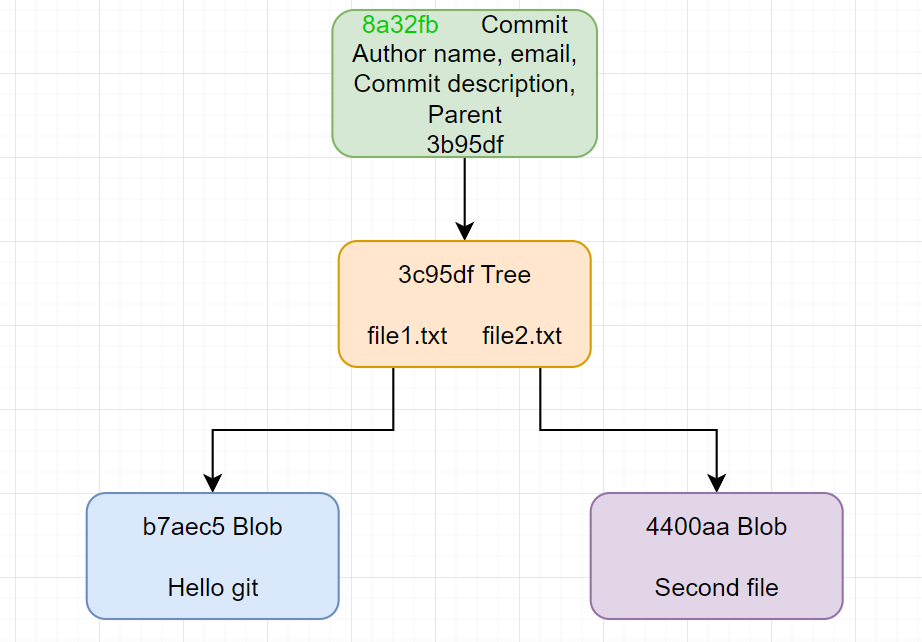
\includegraphics[scale=0.5]{Github/Git_f4.png}
\end{figure}

Como se puede ver, el archivo de versión (commit) es una especie de envoltorio para el objeto tree, y tiene un apuntador hacia el tree. Cada uno de los commits, puede ser llevado al directorio de trabajo para ver esa versión del proyecto. Los siguientes comandos sirven para establecer en git el nombre y dirección de correo electrónico:

\begin{verbatim}
git config --global user.name <name>
git config --global user.email <Email> 
\end{verbatim}

Y para leer la configuración establecida, usamos el siguiente comando: \texttt{git config --list}

\subsection{Creación de las primeras versiones}

En primer lugar, debemos estar pendientes de cuál es el estado del repositorio.

\begin{verbatim}
git status
\end{verbatim}

Con el comando anterior podemos ver los cambios realizados para ser confirmados. También podemos ver si hay algún cambio sin seguimiento para añadir y posteriormente ser enviados/confirmados. 

Una vez tengamos listos los cambios realizados para enviar, usamos el comando \texttt{git commit -m "comment"}. Con la opción \texttt{-m} podemos asignar un comentario a la versión. Es muy importante tener en cuenta que cuando hacemos confirmación de versión, estamos enviando información del 'staging area' al 'git repository', y cuando hacemos el proceso contrario (desde 'staging area' a 'working directory'), el proceso se llama 'checkout'.

El commit como archivo hash contiene lo siguiente:

\begin{itemize}
    \item tree (es el hash del tree principal al que apunta el commit)
    \item parent (es el hash del commit anterior)
    \item Usuario autor de los cambios  
    \item Usuario que confirmó el cambio
    \item Comentario
\end{itemize}

\subsection{Comandos básicos de git}

\begin{itemize}
    \item \texttt{git status}
    \item \texttt{git add} con este se agregan aarchivos al area de staging
    \item \texttt{git commit} con este se se escriben los cambios al repositorio ya como objetos
    \item \texttt{git log} con este se muestra el historial de cambios o commits
    \item \texttt{git checkout} este comando sirve para poner en el directorio actual (working directory) un commit o un branch específico.
    \item \texttt{git cat-file -p <hash>} Con este comando, como se mostró arriba, se visualiza el contenido del archivo correspondiente al hash ingresado.
    \item \texttt{git ls-files -s} Lista todos los archivos (blob) indicando el directorio donde están e indicando su hash.
\end{itemize}



Cuando se agrega un nuevo archivo al directorio, los archivos pueden tener cuatro estados diferentes:
\begin{itemize}
    \item Untracked
    \item Modified
    \item Staged
    \item Unmodified
\end{itemize}


Si un archivo recién creado se adiciona al directorio, directamente está en el estado "untracked". En la siguiente figura se puede observar cómo va cambiando el estado de los archivos.


\begin{figure}[H]
    \centering
    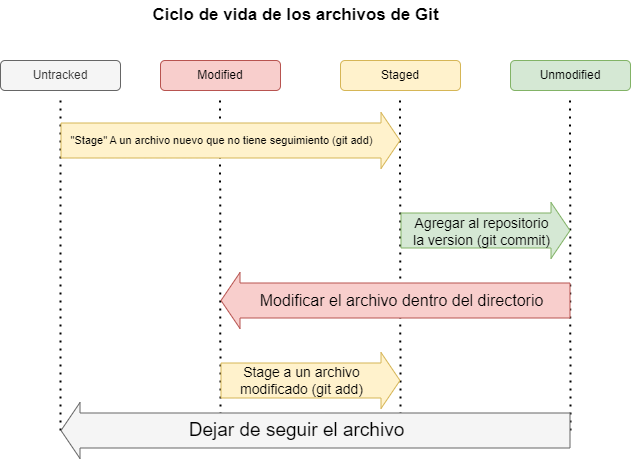
\includegraphics[scale=0.65]{Github/Git_f5.png}
\end{figure}

Para listar los archivos que están dentro del staging area, se usa el comando \texttt{git ls-files -s}. Al agregar archivos al área de staging, tenemos varis opciones

\begin{itemize}
    \item \texttt{git add <name>} Agrega el archivo especificado a la zona de preparación.
    \item \texttt{git add -A} Agrega todos los archivos modificados, eliminados y nuevos al área de preparación. La opción -A incluye archivos en subdirectorios.
    \item \texttt{git add .} solo incluye los archivos en el directorio actual.
    \item \texttt{git add -u} Agrega todos los archivos modificados y eliminados al área de preparación, pero no los nuevos.
    \item \texttt{git add -p} Abre una sesión interactiva que permite agregar solo partes seleccionadas de los cambios realizados en un archivo.
\end{itemize}

Además podemos quitar archivos del area de preparación, mediante el comando \texttt{git rm --cached <name>}, esta última opción sirve para quitar un archivo en específico. \\

Una de las propiedades importantes de ver es que cuando realizamos un commit, este tiene un apuntador a su commit padre, es el hash de su commit padre. Según el tipo de commit este tendrá uno u otro commit padre (más adelante se verá que para pull requests pueden haber punteros distintos.

\subsection{Historial de un archivo}

Un comando útil para analizar la historia de un archivo en nuestro repositorio es el siguiente

\begin{verbatim}
    git log --pretty=oneline <archivo_con_su_ruta>
\end{verbatim}

Este comando retorna una lista de hashes que corresponden a los commits que han modificado dicho archivo:

\begin{verbatim}
13bde112178bbf94d9f83a2a14397c14d8cb973b UpdateBrowser
288cb6fee465de9e1bf682c7b47a25c4c75dd9e7 UpdateBrowser
2f7e1498f72e5d77b2773938f8516dd4c576b922 UpdateDictJson
23835e0a0d35796e708c50cfc71c523ef1b941d5 UpdateDictJson
f9dd3785bbc39a5e1ae9f8fed003f7b696f17f6b Se cambia apertura de navegador para form OVH
e1b1a7f0632ef745d02749468aa02eee016e62f9 Merge branch 'test2' of https://github.com/JhoAraSan/Process into test2
863641d145bdff2d4546a9b8f0328afed95d74ac Update code
47cf1a72d0ee58077a61558072c0866c46295547 cloudflare form bus ixed
673268edaff5d407e7de309c14e8a81829adf137 update
bdc232b7cb40c41c70eacfe7182d510145f26ce2 check bug
.
.
.
\end{verbatim}

Como se puede ver, se muestra el hash del commit y a continuación se muestra el comentario realizado. El primer commit en la lista es el más reciente. El último de la lista será el commit que creó el archivo. 

De forma alternativa, se puede ver solamente el commit creador del archivo en cuestión mediante el comando

\begin{verbatim}
git log --pretty=oneline --diff-filter=A -- .\Consola_3000\Consola3000.py
\end{verbatim}

El cual devuelve

\begin{verbatim}
04bf774da85b9db1a059da4111887240ad2b3d4e renombramiento de carpeta a sugerencia de Sebastian
\end{verbatim}

\section{Las ramas}

Como introducción a la sección, recordemos la capacidad de llevar un commit (screenshot de una versión del proyecto) al directorio actual. Esto se realiza mediante el comando "git checkout". En otras palabras, es algo así como saltar hacia una versión especifica del proyecto. \\

Una definición general de lo que es una rama de github, es que es una referencia textual a un commit. Las siguientes son características de las ramas en git:

\begin{enumerate}
    \item La rama por defecto es la master.
    \item En un mismo repositorio pueden existir varias ramas.
    \item Los apuntadores a todas las ramas se localizan en \texttt{.git/refs/heads}
    \item Cada rama maneja sus propios commits.
    \item El puntero de la rama se mueve automáticamente después de cada nuevo commit.
    \item Para cambiar de branch se usa el comando \texttt{git checkout <branch>}
\end{enumerate}

El puntero de la rama será el último commit realizado en dicha rama, el archivo es un texto que contiene el hash de dicho commit.

\subsection{HEAD}

El concepto de head es util para especificar al sistema cuál es la rama en la que me encuentro actualmente. Básicamente HEAD es el apuntador que apunta hacia la rama/commit \textbf{actual}. Solamente existe un solo HEAD en cada proyecto.

\begin{enumerate}
    \item El puntero se guarda en \texttt{.git/HEAD}
    \item El Puntero por defecto es \texttt{refs:/heads/master}
    \item Para cambiar la referencia a una rama específica se usa \texttt{git checkout <branch>}
    \item Para cambiar la referencia a un commit específico se usa \texttt{git checkout <sha1>}
\end{enumerate}

\begin{figure}[H]
    \centering
    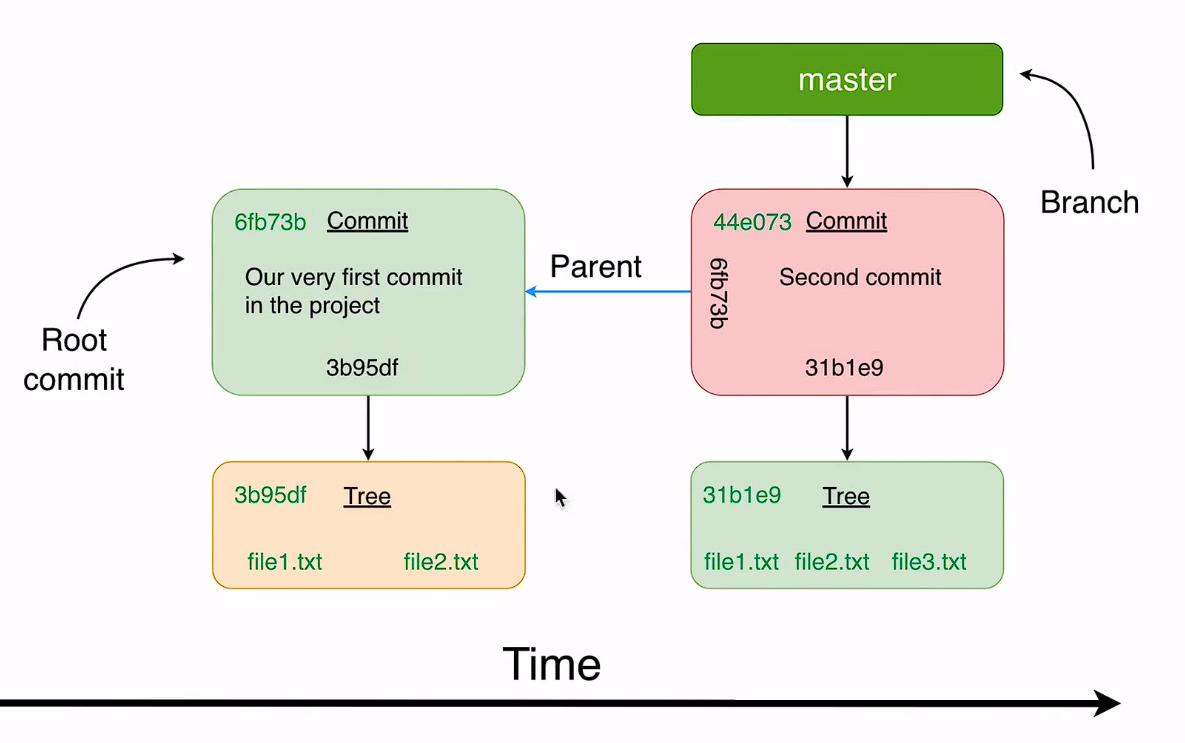
\includegraphics[scale=0.4]{Github/Git_f6.png}
\end{figure}


Cada vez que se crea una nueva rama en un repositorio de Git, se crea una referencia a la cabeza (HEAD) de esa rama en el sistema de archivos de Git. Esta referencia se guarda en el directorio \texttt{.git/refs/heads/} dentro del repositorio.


Para la administración de las ramas disponemos de los siguientes comandos:

 \begin{itemize}
     \item \texttt{git branch} Lista todas las ramas locales
     \item \texttt{git branch <name>} Crea una nueva rama
     \item \texttt{git checkout <branch>} Se dirige a la rama especificada
     \item \texttt{git branch -d <name>} Borrar la rama especificada
     \item \texttt{git branch -m <old> <new>} Renombrar la rama especificada
 \end{itemize}

 Un comando muy útil para crear una rama nueva y dirigirse directamente a ella es la siguiente:

 \begin{verbatim}
git checkout -b <branch name>
 \end{verbatim}

\subsubsection*{Ejemplo}

Para un repositorio de un proyecto cualquiera como ejemplo vamos a la carpeta \texttt{.git/refs/heads}.

Si se lista el contenido del directorio se obtiene la siguiente salida

\begin{verbatim}
    Directory: C:\Users\seb-c\OneDrive\Documentos\Project_Process\Process\.git\refs\heads

Mode                 LastWriteTime         Length Name
----                 -------------         ------ ----
la---           3/25/2023  3:49 PM             41 master
la---            9/6/2023  9:31 AM             41 speechGen
la---           9/10/2023  4:00 PM             41 test2
\end{verbatim}

El cual muestra que en el repositorio de ejemplo hay tres ramas: master, speechGen y test2. Si queremos ver el contenido del archivo \texttt{speechGen} se obtiene

\begin{verbatim}
866c48dd5d96c7ba7ae730dbd3dc85896bc6b576
\end{verbatim}

Este es el hash correspondiente al \textbf{último} commit de esta rama. De aquí se puede concluir que la rama puede verse como un apuntador hacia el commit. 

Para ver dónde se guarda el apuntador general HEAD hacia la rama (o commit) en el que se está actualmente. Vamos al directorio que guarda el puntero: 

\begin{verbatim}
cd .git
cat HEAD
\end{verbatim}

Se obtiene lo siguiente


\begin{verbatim}
ref: refs/heads/test2
\end{verbatim}

El cual indica que en el momento de realizar el comando, el usuario estaba en la rama \texttt{test2}

\section{Repositorios remotos}

En esta sección se describirán algunas características no antes vistas sobre los procesos asociados a los repositorios remotos.

\subsection{git diff}

Este es un comando que puede ser útil para ver y evidenciar las diferencias entre un archivo modificado su anterior versión dentro de la consola. Al usar el comando podemos ver el hash provisional del nuevo archivo (el que tendria si se realiza el commit), las líneas agregadas- quitadas-modificadas.

\section{Fusión o combinación de ramas}
Es importante tener clara la perspectiva de dónde está apuntando \texttt{HEAD}. De ello depende la información que vamos a obtener al llamar al comando \texttt{git log}. Si estamos visualizando commits anteriores, ese commit será el actual para la vista que tengamos en el momento. \\
Ahora teniendo en cuenta lo anterior, suponemos que hemos creado una rama para agregar cualquier especificación; hemos creado esa rama desde la rama principal. Luego hemos realizado cambios en dicha rama y hemos confirmado dichos cambios. Posteriormente volvemos a cambiar la vista hacia la rama principal y \textbf{desde esta rama traemos o unimos los cambios realizados en la rama secundaria}; ese es el proceso de fusión o combinación de ramas. 

\begin{verbatim}
git merge <feature-branch>
\end{verbatim}
En esencia, cuando hacemos la fusión de ramas, lo que estamos realizando es un cambio del apuntador de la rama hacia la que fusionamos (la principal) para apuntar ahora al último commit realizado en la rama que estamos trayendo. Este caso aplica cuando en la rama principal no hay cambios después de haber creado la rama secundaria.\\
\begin{figure}[H]
    \centering
    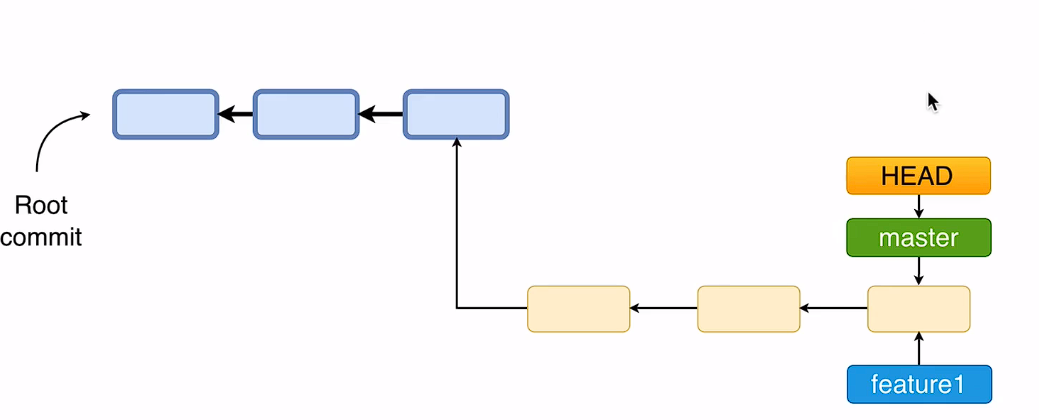
\includegraphics[scale=0.5]{Github/Git_f7.png}
\end{figure}
Supongamos ahora que tenemos nuestra rama principal, creamos una rama para trabajar en características secundarias, pero al mismo tiempo también realizamos cambios en la rama principal. Si en este momento queremos hacer una fusión de las ramas, ya no podemos simplemente cambiar el puntero de la rama principal; ahora es necesario realizar una fusión de 3 direcciones. \\
En la fusión de tres direcciones tenemos tres versiones importantes: la versión ancestro, que corresponde a la última versión en común que tienen las dos ramas a unir; la última versión de la rama secundaria y la última versión de la principal.
Como en la fusión anterior, también se debe ir a la versión de la rama receptora; se crea una nueva versión de fusión en esta rama; \textbf{dicha versión tendrá como versiones padres la última de la rama receptora y la última de la rama secundaria}. Si no existen conflictos entre archivos que se hayan modificado en ambas ramas, simplemente la nueva versión combinará los archivos nuevos.\\

\begin{figure}[H]
    \centering
    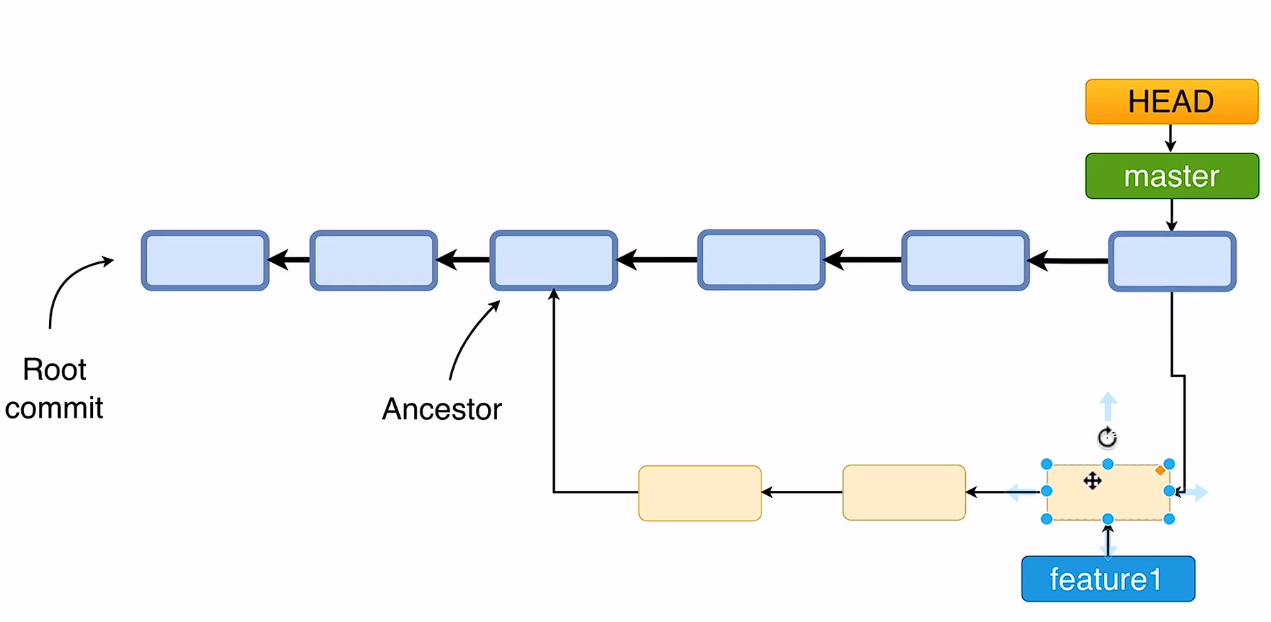
\includegraphics[scale=0.3]{Github/Git_f8.png}
\end{figure}
Una vez realizado este proceso, se puede borrar la rama secundaria, lo cual significa borrar el apuntador de la rama, las versiones permanecen. 

\subsection{conflictos de fusión}

Los conflictos ocurren cuando se intenta fusionar dos ramas y en ambas se ha modificado el mismo archivo. Estos conflictos siempre deben ser arreglados manualmente. Si intentamos unir dos ramas y se generan conflictos, el estado actual del repositorio cambiará a tener dos caminos sin fusionar. Git le pedirá al usuario que corrija los conflictos y que confirme dichos cambios. Están las opciones de dejar los cambios de la rama principal, dejar los cambios de la rama secundaria, o de dejar ambos cambios. \\

Algo interesante de observar, es que en este momento se habrán creado tres objetos blob diferentes en el staging area. tres objetos que tienen el nombre del archivo que contiene el conflicto. El primero corresponde a la versión ancestro de ambas ramas, el segundo corresponde a la modificación de la rama principal, y el ultimo corresponde a la modificación de la rama secundaria. Existen varias formas de resolver estos conflictos; el primero se puede hacer mediante la consola: \\

Abrimos el archivo que contiene los conflictos mediante \texttt{nano} por ejemplo y seleccionar manualmente cuál de la(s) líneas van a ser conservadas. guardar el archivo y de esta manera el o los conflictos habrán sido resueltos. También se tiene a opción de incluso volver a modificar el archivo si ninguna de las dos versiones es la que queremos. Finalmente cuando las modificaciones sean las deseadas, podremos concluir la fusión de las ramas mediante la confirmación (commit). 

\section{Comandos para los repositorios remotos}

Dentro de los comandos más importantes para la clonación de los repositorios remotos, los siguientes son los más importantes:

\subsection{Git push}

Añadido a las tres áreas de los repositorios, tenemos un área adicional que corresponde al repositorio remoto. El primer comando envía toda la información desde el área de repositorio local y lo envía directamente al repositorio remoto. Solamente los cambios que están confirmados son los que efectivamente se ven reflejados en el repositorio remoto. 

\begin{figure}[H]
    \centering
    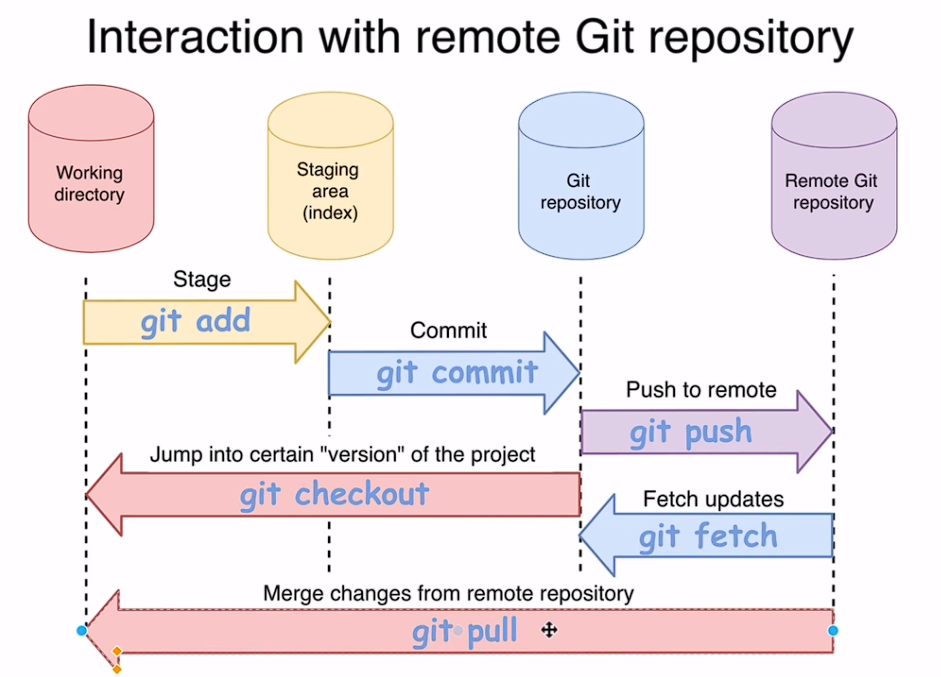
\includegraphics[scale=0.5]{Github/Git_f9.png}
\end{figure}

\subsection{Git fetch y pull}

Una vez el repositorio está actualizado, y es necesario pasar esa información al repositorio local, se pueden hacer dos comandos, el primero es \texttt{git fetch}: este comando es para enviar toda la información del repositorio remoto al repositorio local, pero sin enviarlo al área del directorio de trabajo. Por su parte, si queremos enviar directamente la información del repositorio remoto al directorio de trabajo usamos el comando \texttt{git pull}. \\

Para entender un poco la diferencia entre los dos comandos, supóngase que se crea una nueva rama en el repositorio remoto. Después de realizar \texttt{git fetch} dicha rama será creada en el repositorio local. En otras palabras, con git fetch básicamente estoy actualizando la información del repositorio remoto en mi repositorio local.

Por su parte, el siguiente ejemplo muestra el funcionamiento de \texttt{pull}:

\begin{enumerate}
    \item Se clona el repositorio remoto
    \item Se hace \texttt{checkout} a la rama master en el repositorio local
    \item Se realizan cambios y se confirman en la rama master del repositorio remoto
    \item Después de realizar \texttt{git pull} el repositorio local extraerá los cambios del remoto.
    \item Git realiza la fusión de la rama master en el repositorio local 
    \item Tanto el área de stagig como el directorio de trabajo se actualizan automáticamente luego de la fusión.
\end{enumerate}

Cuando uno clona un repositorio remoto en uno local, git automaticamente crea un enlace entre ambos repositorios. Por defecto para el repositorio local, el nombre del repositorio remoto es \texttt{origin}. 

Siempre que se clona un repositorio, git solamente crea una rama local con el mismo nombre de la rama por defecto del repositorio remoto. Por tanto, si tenemos dos ramas en el repositorio remoto, y clonamos este repositorio, en nuestro repositorio local solamente habrá una rama que es la rama principal del repositorio remoto. Para poder traer una rama remota que no es la principal a nuestro repositorio local, solamente necesitamos hacer un checkout a dicha rama, de esta forma esta rama aparecerá en nuestro repo local.

Para los repositorios remotos, un comando importante y útil puede ser el siguiente \texttt{git remote show origin}. Con este comando podemos ver mucha más información sobre el repositorio remoto como las ramas remotas, las ramas locales, cuáles están configuradas o trackeadas, etc. El siguiente es un ejemplo de la unformación total de un repositorio remoto:

\begin{verbatim}
PS C:\Users\seb-c\OneDrive\Documentos\Project_Process\Process> git remote show origin
* remote origin
  Fetch URL: https://github.com/JhoAraSan/Process.git
  Push  URL: https://github.com/JhoAraSan/Process.git
  HEAD branch: master
  Remote branches:
    master                      tracked
    refs/remotes/origin/clases  stale (use 'git remote prune' to remove)
    refs/remotes/origin/test    stale (use 'git remote prune' to remove)
    refs/remotes/origin/virtual stale (use 'git remote prune' to remove)
    speechGen                   tracked
    test2                       tracked
  Local branches configured for 'git pull':
    master    merges with remote master
    speechGen merges with remote speechGen
    test2     merges with remote test2
  Local refs configured for 'git push':
    master    pushes to master    (up to date)
    speechGen pushes to speechGen (up to date)
    test2     pushes to test2     (up to date)
\end{verbatim}

En este ejemplo "\texttt{stale}" indica que la rama fue borrada del repositorio remoto, y se puede quitar de la lista con el comando \texttt{git remote prune origin}

Por su parte, cuando queremos sincronizar los cambios entre el repositorio remoto y el local, las ramas siempre harán un merge, es decir que se fusionarán y habrá que manejar los posibles conflictos que hayan entre la rama local y su correspondiente remota.  

Para el siguiente ejemplo podemos listar todas las ramas en los repositorios local y remoto:

\begin{verbatim}
git branch -a     

  master
  speechGen
* test2
  remotes/origin/HEAD -> origin/master
  remotes/origin/clases
  remotes/origin/master
  remotes/origin/speechGen
  remotes/origin/test
  remotes/origin/test2
  remotes/origin/virtual
\end{verbatim}

Como se puede ver, la línea \texttt{remotes/origin/HEAD -> origin/master} indica que en el repositorio remoto, la rama por defecto es la master.

\subsection{Ramas rastreadas}

Las ramas rastreadas son todas las ramas del repositorio remoto que tienen su correspondencia con la rama en el repositorio local. En otras palabras, son las ramas que aparecen tanto en el repositorio remoto como en el repositorio local.

Cuando se clona un repositorio remoto, solamente se crea la rama principal en el repositorio local. Estando en repositorio local se realiza el comando \texttt{git checkout} a una rama del repositorio remoto, y en ese momento se crea la rama rastreada. El comando \texttt{git branch -vv} muestra información de las ramas rastreadas:

\begin{verbatim}
git branch -vv

  master    5d42019 [origin/master] Unificando y dejando la verdadera principal
  speechGen 866c48d [origin/speechGen] first ver apps module in window DONE!
* test2     3c3e9ae [origin/test2] Cambio del nombre de la Appstore
\end{verbatim}

Como se ve, se muestra el nombre, el hash y el comentario de las ramas que están rastreadas.

\subsection{Proceso pull}

Para realizar un \texttt{git pull}, se combinan varios conceptos previamente discutidos:

\begin{enumerate}
    \item Rama de reastreo local: Es necesario tener una rama local que esté rastreando una rama remota para poder realizar un \texttt{pull}
    \item Funcionamiento del \texttt{merge}: Es necesario entender cómo funcionan las fusiones. Recordar que puede hacerse con el enfoque de avance rápido o con una fudión de tres vías.
    \item \texttt{git fetch} antes del \texttt{pull}, git efectúa un \texttt{fetch} para obtener todos los cambios desde el repositorio remoto
\end{enumerate}

El proceso de \texttt{git pull} se realiza en dos pasos:\\
Primero se ejecuta un \texttt{git fetch}, que tona todas las actualizaciones del repositorio remoto y las escribe en el repositorio local. Esto incluye todas las nuevas reamas y versiones creadas en el repositorio remoto.

Luego de ejecuta un \texttt{git merge}. Esta fusión es local, es decir, se hace en el repositorio local sin interactuar con el repositorio remoto. Durante este proceso, se utilizan dos ramas: la rama receptora será la rama local y la rama "feature" será la rama remota correspondiente. Git mezclará la rama remota en la rama local. \\
Es relevante notar que Git usa un término especial, "Fetch Head", en lugar del nombre de la rama remota durante este proceso. Como limitación, \texttt{git pull} actualiza solo la rama local que está actualmente en uso. No afecta ninguna otra rama local.


\subsection{Fetch head}

Pongamos un ejemplo: sea un repositorio tal que al revisar las ramas tanto locales como remotas obtenemos el siguiente resultado:

\begin{verbatim}
git branch -a

*   feature-1
    master
    remotes/origin/HEAD -> origin/master
    remotes/origin/master
\end{verbatim}

Vemos que tenemos las dos ramas remotas master y feature-1 con sus correspondientes ramas locales. Si hacemos el siguiente código

\begin{verbatim}
git branch -vv
*   feature-1   ccc9d7b [origin/feature-1] 
    master      f38cf54 [origin/master]
\end{verbatim}

Vemos nuevamente la correspondencia entre las ramas. Escribiendo el comando \texttt{fetch} y luego \texttt{pull} tenemos lo siguiente:

\begin{verbatim}
git fetch -v

From https://github.com/yo/myrepo
 = [up to date] feature-1   ->  origin/feature-1
 = [up to date] master      ->  origin/master

git pull
Already up to date

 
git pull -v
 
From https://github.com/yo/myrepo
 = [up to date] feature-1   ->  origin/feature-1
 = [up to date] master      ->  origin/master 
 Already up to date
 \end{verbatim}

Con lo anterior podemos ver que pull siempre hace fetch antes de hacer algunos cambios adicionales para 
intentar fusionar las ramas.



Si vemos los archivos que están dentro de la carpeta \texttt{.git} podremos ver que hay un archivo llamado \texttt{FETCH\_HEAD}, cuyo contenido sería el siguiente


\begin{verbatim}
cat FETCH_HEAD
73acf27141929dd1f890236317cb54009914c35a                branch 'test2' of https://github.com/JhoAraSan/Process
629fab88a1c5954a9389c827f0e7b4829ce734ba        not-for-merge   tag '1' of https://github.com/JhoAraSan/Process
\end{verbatim}

Este contenido corresponde a las ramas que están en el repositorio remoto. Si cambiamos de rama, al hacer este mismo comando, veremos en primer lugar la rama que está actualmente. Cuando hacemos git pull, Git primero ejecuta "git fetch". Despues del fetch se actualiza la lista de .git/FETCH\_HEAD y la primera rama de esta lista será la rama actual. 
finalmente Git ejecuta \texttt{git merge FETCH\_HEAD} que busca la primera rama en el fetch head sin la etiqueta "not-for-merge" y la fusiona con la rama local actual. 

\subsection{Git pull con modificacion de repositorio remoto}

Si despues de hacer \texttt{git pull} el repositorio remoto es modificado, se crea un nuevo commit en el repositorio remoto. Git actualiza el repositorio y realiza la actualización del apuntador en el repositorio local, del commit antiguo al nuevo commit. \\

Ahora supongamos que se realizan cambios tanto en el repositorio remoto como en el repositorio local, y queremos traer o hacer pull al repositorio remoto. Tengamos en cuenta que al revisar con \texttt{git log}, veremos el último commit que acabamos de hacer, y anterior a ese veremos el último commit sincronizado; el que se supone que es el último commit del repositorio remoto. Sabemos que esta es una información falsa, pues este commit está desactualizado. Mediante el comando \texttt{git fetch}, vamos a actualizar la información del cambio realizado en el repositorio remoto, aunque Git ya creó los objetos dentro del repositorio local, estos aún no se ven en el directorio de trabajo porque aún no se ha fusionado con la rama local.

Después de esto podemos fusionar el cambio remoto con el cambio local. Mediante \texttt{git merge FETCH\_HEAD} 

\subsection{Subida de cambios al repositorio remoto}

Ahora que tenemos cambios en el repositorio local que están ausentes en el repositorio remoto, es hora de poner la operación push en acción. Recordar siempre que es necesario tener permisos de escritura. Una vez estén sincronizados los repositorios, podemos ver que los apuntadores de los repositorios local (que está en la carpeta \texttt{.git/refs/head}) y la remota (que está en la carpeta \texttt{.git/refs/remotes/origin}) tienen el mismo c0ommit de destino. \\

Si necesitamos crear una rama nueva, los pasos a realizar para que también se vea reflejada en el repositorio remoto es lo siguiente:

\begin{enumerate}
    \item Se crea la nueva rama local mediante \texttt{git checkout -b nueva}
    \item Se hacen los cambios correspondientes.
    \item Se confirman los cambios con \texttt{commit}
    \item Se sube la nueva rama al repositorio remoto con el comando \texttt{git push -v -u origin feature-2}
\end{enumerate}

\subsection{De rama local a rama nueva remota}

Cuando se crea una rama nueva en el repositorio local y se requiere tener dicha rama en el repositorio remoto es necesario crear la rama nueva en ambos lados de forma manual. Si intentamos ejecutar el comando \texttt{push} a una rama nueva que no está en el repositorio remoto, obtendríamos el siguiente error:

\begin{verbatim}
fatal: The current branch nombre has no upstream branch.}
To push the current branch and set the remote as upstream, use
    git push --set-upstream origin nombre
\end{verbatim}

el comando sugerido \texttt{git push --set-upstream origin nombre} efectivamente realiza la creación de la rama. Sin embargo, un comando equivalente y más corto es el siguiente

\begin{verbatim}
git push -v -u origin nombre
\end{verbatim}

Y así queda creada la rama en el repositorio remoto con el mismo nombre que la rama local nueva. 


\subsection{Actualización de estados de ramas}

Cuando una rama del repositorio remoto se elimina, es necesario realizar una actualización en el repositorio local. Si se ejecuta el comando \texttt{git branch -vv} se observará que aunque en el repositorio remoto ya no exista, la rama local todavía sigue a la rama remota. Incluso después de actualizar el repositorio mediante \textit{git fetch}, vemos que la rama sigue siguiendo a la desaparecida rama remota. 
Para este caso se usa el siguiente comando

\begin{verbatim}
git remote update origin --prune
\end{verbatim}
Esto asegura que el repositorio local reconozca la eliminación de la rama remota. Finalmente se ejecuta 
\texttt{git branch -D nombre}. Para eliminar también la rama local.

Ahora, también es posible eliminar la rama remota desde la consola local:

Recordemos que cuando se crea una nueva rama local, se debe especificar al momento de publicar el repositorio remoto:

\begin{verbatim}
git push -u origin nombre-rama
\end{verbatim}
El comando para borrar una rama remota es 

\begin{verbatim}
git push origin -d nombre-rama
\end{verbatim}
Y luego se borra la rama local

\begin{verbatim}
git branch -D nombre-rama
\end{verbatim}

\subsubsection{comando \texttt{git show-ref}} Este comando es putil porque indica todas las referencias a las correspondientes versiones de las ramas tanto locales como remotas:

\begin{verbatim}
git show-ref     
5d42019b30082902c9dd6dc8ebfcb5f63c75095d refs/heads/master
866c48dd5d96c7ba7ae730dbd3dc85896bc6b576 refs/heads/speechGen
4b8c370d8bbe8d2769cdb69e91d90fc9a2a7338e refs/heads/test2
5d42019b30082902c9dd6dc8ebfcb5f63c75095d refs/remotes/origin/HEAD
5d42019b30082902c9dd6dc8ebfcb5f63c75095d refs/remotes/origin/master
866c48dd5d96c7ba7ae730dbd3dc85896bc6b576 refs/remotes/origin/speechGen
4b8c370d8bbe8d2769cdb69e91d90fc9a2a7338e refs/remotes/origin/test2
d5c7ebc8c4cdf48f3395a092f5616a33f0aab274 refs/stash
\end{verbatim}

Es un indicador muy útil para saber si un repositorio está debidamente actualizado. El comando puede especificar una sola rama solo añadiendo el nombre de la misma al comando.

\section{Pull Requests}

Una manera de definir las peticiones o solicitudes de integración "Pull requests" sería la siguiente:
Una solicitud de integración es una propuesta de potenciales cambios en el repositorio. La idea principal detrás de trabajar con Git es desarrollar múltiples características de manera simultánea, usualmente en diferentes ramas y por diferentes personas. Cuando un colaborador, como Bob o Mike, está listo para aplicar cambios a la rama principal, inician comunicación con otros desarrolladores a través de "pull requests". Un "pull request" es simplemente una propuesta de cambios potenciales en el código. Estos cambios son "potenciales" porque después de una revisión por parte de otros desarrolladores, pueden ser rechazados o aprobados. Si se rechazan, el "pull request" se cierra y la rama correspondiente se elimina. El objetivo principal es aplicar los cambios para avanzar en el desarrollo.

El término "Pull Request" o "Merge Request" depende del contexto y del flujo de trabajo en desarrollo de software. En un entorno donde todos los desarrolladores trabajan en el mismo repositorio y tienen acceso de escritura, "Merge Request" sería más apropiado porque el objetivo es fusionar cambios en la rama principal tras la aprobación de revisores.

En cambio, en proyectos de código abierto con múltiples repositorios (uno principal y otros bifurcados), "Pull Request" es más adecuado. Aquí, un desarrollador que no tiene acceso de escritura al repositorio principal puede solicitar que el propietario del repositorio principal "jale" y revise los cambios de una rama en un repositorio bifurcado.

Por lo tanto, si los desarrolladores trabajan en el mismo proyecto, "Merge Request" es más apropiado. Si los desarrolladores crean bifurcaciones del repositorio y el propietario debe jalar cambios de esas bifurcaciones, entonces "Pull Request" es más adecuado.

\subsection{Paso a paso del proceso de solicitudes de integración}

El siguiente ejemplo expone de manera clara el proceso.

En un flujo de trabajo de desarrollo, dos desarrolladores, Mike y Bob, colaboran en un proyecto. Mike crea una nueva rama llamada "feature-one" en su computadora local y realiza cambios. Una vez satisfecho, sube estos cambios al repositorio remoto. A continuación, abre un "Pull Request" para iniciar el proceso de revisión por parte de otros colaboradores. Él puede iniciar el proceso de solicitud de integración una vez su rama esté en el repositorio remoto.

Mike solicita a Bob revisar esta solicitud. Él puede añadir dentro de la petición algunas descripciones de los cambios que realizó en su rama. Bob puede optar por descargar la rama para probar los cambios localmente o revisarlos directamente en línea. Tras la revisión, Bob puede añadir comentarios o solicitar cambios adicionales. Mike puede hacer los cambios necesarios y actualizar el Pull Request existente sin necesidad de crear uno nuevo. El Pull Request se actualiza automáticamente cuando él confirma los cambios en su rama y los sube al repositorio remoto.  Cuando estas actualizaciones son subidas, a Bob se le notifica mediante correo electrónico sobre las nuevas versiones.

Una vez que Bob aprueba los cambios y se alcanza el número requerido de aprobaciones, se permite la fusión del Pull Request en la rama principal. Dependiendo de los permisos, uno de los desarrolladores o un administrador realiza la fusión.

Este proceso permite la colaboración efectiva y revisiones detalladas antes de que los cambios se integren en las ramas principales del proyecto. En resumen, el Pull Request es una herramienta central para revisar e implementar características en un entorno de desarrollo colaborativo.

Dentro de la página del repositorio remoto está la opción para crear una nueva solicitud de integración. Es importante que para que pueda haber una fusión, no pueden haber conflictos de fusión, por tanto cualquier conflicto de fusión debe resolverse antes de iniciara la solicitud de integración.

En la creación de la solicitud de integración se deber realizar una descripción del cambio, actualización, componente, característica, etc, realizado. Siempre es recomendable realizar la mejor descripción posible, ser muy claro y conciso con la descripción. 

Una vez creada la solicitud, las personas pueden revisarla, añadir comentarios, ver los cambios que se han realizado, etc. Por ejemplo, dentro de la pestaña de archivos modificados, uno puede insertar un comentario sobre una línea de código específica. 

Existen dos opciones para publicar el comentario: uno es añadir un solo comentario a la línea de código, y la otra es iniciar una review, que implica un grupo de líneas o una sección de código. Por otro lado está la opción de aprobar la solicitud dejando un comentario de la aprobación,  dejar un simple comentario sin indicar aprobación o declinación, y sugerir más cambios para una nueva revisión.

Una vez la solicitud está aprobada, cualquier usuario con los permisos correspondientes puede fusionar la rama. Es importante notar que en algunas ocasiones Github por defecto permite a usuarios fusionar la rama incluso si no hay ninguna review. 